\documentclass[a4paper, justified]{tufte-handout}
\usepackage{hyperref}
\usepackage{units}
\usepackage{microtype}
\usepackage{tikz}

\usepackage{listings}
\usepackage{xcolor}
\definecolor{maroon}{cmyk}{0, 0.87, 0.68, 0.32}
\definecolor{halfgray}{gray}{0.55}
\definecolor{ipython_frame}{RGB}{207, 207, 207}
\definecolor{ipython_bg}{RGB}{247, 247, 247}
\definecolor{ipython_red}{RGB}{186, 33, 33}
\definecolor{ipython_green}{RGB}{0, 128, 0}
\definecolor{ipython_cyan}{RGB}{64, 128, 128}
\definecolor{ipython_purple}{RGB}{170, 34, 255}

\lstset{
    breaklines=true,
    %
    extendedchars=true,
    literate=
    {á}{{\'a}}1 {é}{{\'e}}1 {í}{{\'i}}1 {ó}{{\'o}}1 {ú}{{\'u}}1
    {Á}{{\'A}}1 {É}{{\'E}}1 {Í}{{\'I}}1 {Ó}{{\'O}}1 {Ú}{{\'U}}1
    {à}{{\`a}}1 {è}{{\`e}}1 {ì}{{\`i}}1 {ò}{{\`o}}1 {ù}{{\`u}}1
    {À}{{\`A}}1 {È}{{\'E}}1 {Ì}{{\`I}}1 {Ò}{{\`O}}1 {Ù}{{\`U}}1
    {ä}{{\"a}}1 {ë}{{\"e}}1 {ï}{{\"i}}1 {ö}{{\"o}}1 {ü}{{\"u}}1
    {Ä}{{\"A}}1 {Ë}{{\"E}}1 {Ï}{{\"I}}1 {Ö}{{\"O}}1 {Ü}{{\"U}}1
    {â}{{\^a}}1 {ê}{{\^e}}1 {î}{{\^i}}1 {ô}{{\^o}}1 {û}{{\^u}}1
    {Â}{{\^A}}1 {Ê}{{\^E}}1 {Î}{{\^I}}1 {Ô}{{\^O}}1 {Û}{{\^U}}1
    {œ}{{\oe}}1 {Œ}{{\OE}}1 {æ}{{\ae}}1 {Æ}{{\AE}}1 {ß}{{\ss}}1
    {ç}{{\c c}}1 {Ç}{{\c C}}1 {ø}{{\o}}1 {å}{{\r a}}1 {Å}{{\r A}}1
    {€}{{\EUR}}1 {£}{{\pounds}}1
}

\lstdefinelanguage{iPython}{
    morekeywords={access,and,break,class,continue,def,del,elif,else,except,exec,finally,for,from,global,if,import,in,is,lambda,not,or,pass,print,raise,return,try,while,yield},%
    %
    % Built-ins
    morekeywords=[2]{abs,all,any,basestring,bin,bool,bytearray,callable,chr,classmethod,cmp,compile,complex,delattr,dict,dir,divmod,enumerate,eval,execfile,file,filter,float,format,frozenset,getattr,globals,hasattr,hash,help,hex,id,input,int,isinstance,issubclass,iter,len,list,locals,long,map,max,memoryview,min,next,object,oct,open,ord,pow,property,range,raw_input,reduce,reload,repr,reversed,round,set,setattr,slice,sorted,staticmethod,str,sum,super,tuple,type,unichr,unicode,vars,xrange,zip,apply,buffer,coerce,intern},%
    %
    sensitive=true,%
    morecomment=[l]\#,%
    morestring=[b]',%
    morestring=[b]",%
    %
    morestring=[s]{'''}{'''},% used for documentation text (mulitiline strings)
    morestring=[s]{"""}{"""},% added by Philipp Matthias Hahn
    %
    morestring=[s]{r'}{'},% `raw' strings
    morestring=[s]{r"}{"},%
    morestring=[s]{r'''}{'''},%
    morestring=[s]{r"""}{"""},%
    morestring=[s]{u'}{'},% unicode strings
    morestring=[s]{u"}{"},%
    morestring=[s]{u'''}{'''},%
    morestring=[s]{u"""}{"""},%
    %
    % {replace}{replacement}{lenght of replace}
    % *{-}{-}{1} will not replace in comments and so on
    literate=
    {á}{{\'a}}1 {é}{{\'e}}1 {í}{{\'i}}1 {ó}{{\'o}}1 {ú}{{\'u}}1
    {Á}{{\'A}}1 {É}{{\'E}}1 {Í}{{\'I}}1 {Ó}{{\'O}}1 {Ú}{{\'U}}1
    {à}{{\`a}}1 {è}{{\`e}}1 {ì}{{\`i}}1 {ò}{{\`o}}1 {ù}{{\`u}}1
    {À}{{\`A}}1 {È}{{\'E}}1 {Ì}{{\`I}}1 {Ò}{{\`O}}1 {Ù}{{\`U}}1
    {ä}{{\"a}}1 {ë}{{\"e}}1 {ï}{{\"i}}1 {ö}{{\"o}}1 {ü}{{\"u}}1
    {Ä}{{\"A}}1 {Ë}{{\"E}}1 {Ï}{{\"I}}1 {Ö}{{\"O}}1 {Ü}{{\"U}}1
    {â}{{\^a}}1 {ê}{{\^e}}1 {î}{{\^i}}1 {ô}{{\^o}}1 {û}{{\^u}}1
    {Â}{{\^A}}1 {Ê}{{\^E}}1 {Î}{{\^I}}1 {Ô}{{\^O}}1 {Û}{{\^U}}1
    {œ}{{\oe}}1 {Œ}{{\OE}}1 {æ}{{\ae}}1 {Æ}{{\AE}}1 {ß}{{\ss}}1
    {ç}{{\c c}}1 {Ç}{{\c C}}1 {ø}{{\o}}1 {å}{{\r a}}1 {Å}{{\r A}}1
    {€}{{\EUR}}1 {£}{{\pounds}}1
    %
    {^}{{{\color{ipython_purple}\^{}}}}1
    {=}{{{\color{ipython_purple}=}}}1
    %
    {+}{{{\color{ipython_purple}+}}}1
    {*}{{{\color{ipython_purple}$^\ast$}}}1
    {/}{{{\color{ipython_purple}/}}}1
    %
    {+=}{{{+=}}}1
    {-=}{{{-=}}}1
    {*=}{{{$^\ast$=}}}1
    {/=}{{{/=}}}1,
    literate=
    *{-}{{{\color{ipython_purple}-}}}1
     {?}{{{\color{ipython_purple}?}}}1,
    %
    identifierstyle=\color{black}\ttfamily,
    commentstyle=\color{ipython_cyan}\ttfamily,
    stringstyle=\color{ipython_red}\ttfamily,
    keepspaces=true,
    showspaces=false,
    showstringspaces=false,
    %
    rulecolor=\color{ipython_frame},
    frame=single,
    frameround={t}{t}{t}{t},
    framexleftmargin=6mm,
    numbers=left,
    numberstyle=\tiny\color{halfgray},
    %
    %
    backgroundcolor=\color{ipython_bg},
    %   extendedchars=true,
    basicstyle=\small,
    keywordstyle=\color{ipython_green}\ttfamily,
}

\usepackage{ifxetex}
\ifxetex
  \renewcommand{\textls}[2][5]{%
    \begingroup\addfontfeatures{LetterSpace=#1}#2\endgroup
  }
  \renewcommand{\allcapsspacing}[1]{\textls[15]{#1}}
  \renewcommand{\smallcapsspacing}[1]{\textls[10]{#1}}
  \renewcommand{\allcaps}[1]{\textls[15]{\MakeTextUppercase{#1}}}
  \renewcommand{\smallcaps}[1]{\smallcapsspacing{\scshape\MakeTextLowercase{#1}}}
  \renewcommand{\textsc}[1]{\smallcapsspacing{\textsmallcaps{#1}}}
  \usepackage{fontspec}
  \setmainfont{Hoefler Text}
  \setsansfont{Gill Sans}[Scale=MatchUppercase]
\fi

\title{Generating text with reinforcement learning}
\author{Maximilian Balthasar Mansky}
\date{\today}
\begin{document}
\maketitle

\section{Goal of this project}

Machine learning approaches to text generation try to replicate a given text, for example by predicting the next word for a sentence. While the results can be interesting, this approach has obvious limitations.\cite{Lau2020} Text can also be generated from structured information, such as information about somebody's life.\cite{lebret2020} These approaches have the drawback that the machines only learns to imitate, in the sense that it reduces the distance between the generated text and the truth. This well-put in an article by Karpathy\cite{karpathy2015} and its response\cite{goldberg2015}. In this project, I want to explore whether a reinforcement learning approach provides different results.

Instead of attempting to generate text by imitation, we can check a generated solution for its correctness. This is done by implementing grammar, vocabulary and further checks in the environments that the machine interacts with. As an example, part of the environment might be responsible for evaluating word order, another for measuring word variations. Text is useful because it is easily verified by humans, compared to game solving strategies. It also allows for a wide variety of possible solutions. "The quick brown fox jumps over the lazy dog" is equally grammatically valid as "the lazy dog is jumped over by the quick brown fox".

\section{Implementation}

There are two parts to reinforcement learning, the agent and an environment. The agent interacts with the environment and receives feedback from it. Conversely, the environment receives input from the agent to change and evaluates the new state. The result of the evaluation is passed back to the agent and forms the basis for its learning.

A simple example is a state environment. Consider a five-state environment, consisting of a negative reward state, a positive reward state, two intermediary and a starting state. 

\begin{marginfigure}
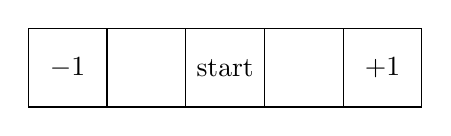
\begin{tikzpicture}
\foreach \i in {0, ..., 4} {
	\draw (\i, 0) rectangle +(1,1) +(0.5, 0.5) node (state \i) {};
	};
\draw (state 0) node {$-1$};
\draw (state 4) node {$+1$};
\draw (state 2) node {start};
\end{tikzpicture}
\caption{A simplified example of an environment. The agent starts in the center cell and can move left or right. The left-most cell contains a negative reward (denoted by $-1$), the rightmost one a positive reward ($+1$).}
\end{marginfigure}

The agent then chooses its actions based on its current state. Possible actions are left or right (It is left to the environment to decide whether a state change is valid. Going left on the left-most cell is often interpreted as not changing state.) and the agent is given information about the result of that change (nil for changing to one of the center states, $\pm1$ for the outermost ones). How the agent learns is dependant on its implementation (i.e. whether it keeps a history, how the initial interaction is treated, how learning is implemented...). The environment is only responsible for evaluating the actions, the agent is responsible from learning from the feedback.

\subsection{Environment}

In this project, the Environment needs to check whether the current state (a text or sentence to be built by the agent) is correct and assign some form of feedback based on it. Each item of correctness will be implemented separately in grammar model. Possible models are:
\begin{itemize}
\item{Sentence length}
\item{Presence of nouns, adjectives, verbs}
\item{Position of words}
\item{Word order/grammatical correctness}
\item{Sentence variation}
\end{itemize}
As current agent learning frameworks can only work with a single reward dimension, the model output must be coerced into a single output by the Environment. It may be worthwhile to explore whether gradually returning the reward from more complex grammar models\footnote{Implementation idea: Use some form of weighted average from the outputs. In the beginning the model may focus on producing sentences of the right length and with a bit of variation ($80\%$ sentence length, $20\%$ word presence) and as learning progresses, focus more on the higher end of complexity ($20\%$ word position, $30\%$ word order, $50\%$ sentence variation).} is useful in guiding the agent. For evaluating the states, the Environment must at least keep track of the current sentence. In this context, a state means a particular sentence, not the individual words.

Within a state, words itself need to be encoded somehow. Either by using a one-hot encoding (limited to the most common words) or a small word2vec model based on a text. The latter has the advantage that the size of the vocabulary can be smoothly increased, by adding more words near to similar ones. In the latter case of a word2vec encoding, it probably also makes sense to include some sort of word accuracy reward, indicating how close the chosen word vector is to the vector output of the agent.

The actions changing states can be implemented in several ways. Either by generating a new state from scratch (that is, the agent generates a sentence for evaluation) or by manipulating the existing state, for example by changing the current word or the ones next to it. An action would consist of two parts: Deciding which to manipulate (current word, previous or next one or quit/finish sentence\footnote{Maybe it is worthwhile to also include insertion of words? Or just move, do not change word?}) and choosing which word to use.

\begin{figure}
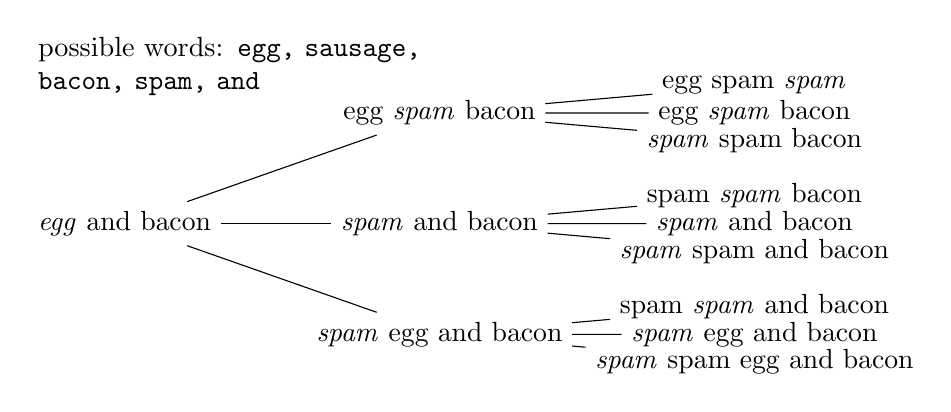
\begin{tikzpicture}[grow=right, level 1/.style={sibling distance=4em},
level 2/.style={sibling distance=1em}, level distance=4cm]]
\coordinate (possible states) at (0,0);
\coordinate (tree root add) at (0,-2);
\draw (possible states) node[anchor = west, text width = 5cm] {possible words: \texttt{egg, sausage, bacon, spam, and}};

\draw (tree root add) node[anchor=west] {\emph{egg} and bacon}
	child {node {\emph{spam} egg and bacon}
		child {node {\emph{spam} spam egg and bacon}}
		child {node {\emph{spam} egg and bacon}}
		child {node {spam \emph{spam} and bacon}}
		}
	child {node {\emph{spam} and bacon}
		child {node {\emph{spam} spam and bacon}}
		child {node {\emph{spam} and bacon}}
		child {node {spam \emph{spam} bacon}}
		}
	child {node {egg \emph{spam} bacon}
		child {node {\emph{spam} spam bacon}}
		child {node {egg \emph{spam} bacon}}
		child {node {egg spam \emph{spam}}}
		};
\end{tikzpicture}
\caption{Example of state transfer from an initial sentence, with the possible words replacements indicated by \emph{emphasized} text.}
\end{figure}
Moving between states can give different paths to the same state (for example "spam spam bacon"), but the reward derived from it should be the same.\footnote{The Environment is ignorant of its previous states and keeps no memory.} 


\begin{thebibliography}{99}
\bibitem{lebret2010} Lebret, Grangier, Auli: \emph{Neural Text Generation from Structured Data with Application to the Biography Domain} \url{https://research.fb.com/wp-content/uploads/2017/02/neural-text-generation-emnlp-camera-ready.pdf}
\bibitem{Lau2020} Lau, Cohn, Baldwin, Hammond \emph{This AI Poet Mastered Rhythm, Rhyme, and Natural Language to Write Like Shakespeare} \url{https://spectrum.ieee.org/artificial-intelligence/machine-learning/this-ai-poet-mastered-rhythm-rhyme-and-natural-language-to-write-like-shakespeare}
\bibitem{karpathy2015} Karpathy: \emph{The Unreasonable Effectiveness of Recurrent Neural Networks} \url{http://karpathy.github.io/2015/05/21/rnn-effectiveness/}
\bibitem{goldberg2015} Goldberg, \emph{The unreasonable effectiveness of Character-level Language Models}\url{https://nbviewer.jupyter.org/gist/yoavg/d76121dfde2618422139}
\end{thebibliography}
\end{document}
